\chapter{STP Tree Generator}
\label{stp-gen}
We split the application in three parts:
\begin{itemize}
    \item \textbf{Client}: collects STP information and sends it to the server.
        The client also handles piecing together the packets into paths.
    \item \textbf{Server}: saves the data from the clients and combines them into one tree.
    \item \textbf{Parser}: contacts the server to receive the tree and converts it into output format.
\end{itemize}
The intended form of usage is to have multiple clients in the network connecting to one server.
We combine information received from multiple clients to reach a better understanding of the network.

STP uses only local data, which means that bridges have no knowledge of the network, except for their own port states.
Unfortunately, this makes it hard to find connections between bridges.
The only way to obtain this information is by capturing packets during the tree build up.

When the client witnesses the message age increasing, it assumes the new root to be prepended to the previous one.
This assumption is uncertain, as this connection cannot be guaranteed, but the risk of making mistakes can be reduced.
Details on this are discussed in the section on uncertain assumptions (Section~\ref{uncertain_assumptions})
Figure~\ref{fig:build_up} shows a rudimentary example of information gained during tree build up.
%TODO: check that the figures don't break any listings
\begin{figure}[p]
    \begin{centering}
        \begin{subfigure}[b]{0.4\textwidth}
            \centering
            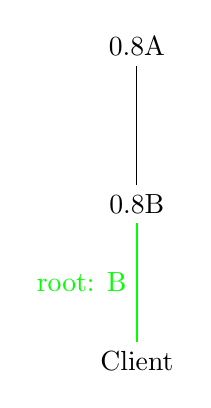
\begin{tikzpicture}
                \node (a) at (4,4) {\switch{0.8}{A}};
                \node (b) at (4,2) {\switch{0.8}{B}};
                \node (client) at (4,0) {Client};

                \draw[green, thick]
                (b) -- node [left] {root: B} ++ (client);
                \draw
                (a) -- (b);

            \end{tikzpicture}
            \caption{B thinks it is root}
        \end{subfigure}
        \hspace{1cm}
        \begin{subfigure}[b]{0.4\textwidth}
            \centering
            \begin{tikzpicture}
                \node (a) at (4,4) {\switch{0.8}{A}};
                \node (b) at (4,2) {\switch{0.8}{B}};
                \node (client) at (4,0) {Client};

                \draw[green, thick]
                (a) -- node [right] {root: A} ++ (b);
                \draw[green, thick] 
                (b) -- node [right] {root: A} ++ (client);

                \begin{customlegend}[legend cell align=left, legend entries={Known Connection, Unknown Connection},
                    legend style={at={(10,4)},font=\footnotesize}]
                    \addlegendimage{draw=green}
                    \addlegendimage{draw=black}
                \end{customlegend}
            \end{tikzpicture}
            \caption{B updates its root information}
        \end{subfigure}
    \end{centering}
    \caption{Information gained on STP build up}
    \label{fig:build_up}
\end{figure}

We only assume network growth for the cases where the message age increases at the same time that the root changes.
For other cases (message age decreasing or staying constant) we did not find ways to gain knowledge about the network.
Without a reason to assume a \textit{certain} network topology, and with the guarantee that the current assumption is incorrect (due to a network change), the client clears its data when witnessing such a change.
Figure \ref{fig:information_lost} shows an example case where the client has to reset its data.
A detailed explanation of how \tool\ handles incoming STP packets can be found in the section on packet handling (Section~\ref{packet_handling}).

\begin{figure}[p]
    \begin{centering}
        \begin{subfigure}[b]{0.4\textwidth}
            \begin{tikzpicture}
                \node (A) at (4,8) {\switch{0.8}{A}};
                \node (B) at (2,6) {\switch{0.8}{B}};
                \node (C) at (6,6) {\switch{0.8}{C}};
                \node (D) at (4,4) {\switch{0.8}{D}};
                \node (client) at (4,2) {Client};

                \draw[thick, draw=green]
                (A) -- (B)
                (B) -- (D)
                (D) -- (client);

            \end{tikzpicture}
            \caption{Some information known}
        \end{subfigure}
        \hspace{1cm}
        \begin{subfigure}[b]{0.4\textwidth}
            \begin{tikzpicture}
                \node (A) at (4,8) {\switch{0.8}{A}};
                \node (B) at (2,6) {\switch{0.8}{B}};
                \node (C) at (6,6) {\switch{0.8}{C}};
                \node (D) at (4,4) {\switch{0.8}{D}};
                \node (client) at (4,2) {Client};

                \draw[thick, draw=green]
                (C) -- (D)
                (D) -- (client);

                \draw[thick, draw=red]
                (A) -- (B)
                (B) -- (D);

                \begin{customlegend}[legend cell align=left, legend entries={Known Information, Lost Information},
                    legend style={at={(8.2,8),font=\footnotesize}}]
                    \addlegendimage{draw=green}
                    \addlegendimage{draw=red}
                \end{customlegend}
            \end{tikzpicture}
            \caption{Previous information lost}
        \end{subfigure}
        \caption{Information lost during tree build up}
        \label{fig:information_lost}
    \end{centering}
\end{figure}

\section{Class Structure}
\label{data}
The classes we created made saving the STP data easier and reduced the effort needed to generate the \textit{JSON} and \textit{TikZ} output.
We created classes to represent MAC addresses, bridges, and complete spanning trees.
All these classes have conversion functions from and to \textit{JSON} format, as well as a function to generate \textit{TikZ} output.
Altogether the following classes were created:
\begin{itemize}
    \item \textbf{Mac}: A container class for MAC addresses.
        It is used to store the address in cleaner format.
    \item \textbf{Bridge}: Stores a \textbf{MAC} object in conjunction with the priority and message age.
    \item \textbf{SpanningTree}: This class represents an entire tree.
        It has functions for creating the \textit{TikZ} export as well as combining and manipulating subtrees.
        The \textbf{SpanningTree} class is a recursive data structure, storing the root as a \textit{Bridge} object and its children as a vector of \textbf{SpanningTree} objects.
        As it is the most important and also the most complex class, the header file is shown in detail in Listing~\ref{lst:spanningTree}.
    \item \textbf{Sniffer}: Does the actual packet sniffing.
    \item \textbf{Client}: Handles the client side communication.
    \item \textbf{Server}: Handles the server side communication, as well as combining the trees and removing incorrect information.
\end{itemize}
\lstinputlisting[caption=The \textbf{SpanningTree} header file, label=lst:spanningTree]{../listings/stp/spanningTree.cpp}
The STP data is saved in the \textbf{Sniffer} as a vector.
This is easier than storing them in a fixed size array, and already combining them into a \textbf{SpanningTree} object would keep the server from performing the steps described in Section~\ref{uncertain_assumptions}.

\section{Packet Handling}
\label{packet_handling}
Packets are handled by the sniffer class.
While the function mostly skips unused fields in the STP packet, here we will take a close look at the more important parts.
In order to check if the packet is actually an STP packet, we use the Ethernet destination address.
Listing~\ref{lst:filter} shows how that is done.
The \textit{bytes} variable is provided by the required \textit{pcap} callback prototype (see Section~\ref{pcap}: PCAP).
This way is computationally more expensive than saving the destination in binary format and comparing memory.
It is however also more readable and a lot easier to change should the need arise.
The address we compare the destination to is the broadcast target for STP.
\lstinputlisting[caption=Filtering for STP packets, label=lst:filter]{../listings/stp/stpFilter.c}

\textit{Pcap} provides us with a pointer to the binary packet data.
We can go through the packet by incrementing this pointer by set amounts (after skipping to the STP data).
This repeats for the bridge identifier, as well as other fields.
Listing~\ref{lst:payload} shows the beginning of the payload handling.
\lstinputlisting[caption=Going Through the Payload, label=lst:payload]{../listings/stp/payload.c}

After the data is extracted from the packet, it is constructed into our custom classes.
We then check if the two bridges (root and first hop) were previously known, as seen in Listing~\ref{lst:contained}.
Concerning the root, knowing whether or not it was previously known is enough.
For the first hop, we also require knowledge about the old message age.
\lstinputlisting[caption=Checking for Previously Known Information, label= lst:contained]{../listings/stp/contained.c}

Listing~\ref{lst:update} shows how we update the bridge information in the sniffer.
The \textit{clearAndAdd} function is just a shorthand to clear the bridge vector before adding the two bridges to it.
\lstinputlisting[caption=Bridge Data Update, label=lst:update]{../listings/stp/update.c}
\section{Communication}
\label{communication}
Our distributed architecture is hierarchical, as we have a distinct \textit{client-server} separation.
We also used a \textit{push} style communication, meaning the clients will "push" their messages to the server, who simply waits for incoming connections.
The alternative would be to have the server poll the registered clients for their data.
This would have doubled the communication effort needed and made the handling for disconnected clients more complicated.
For these reasons that we chose not to do this.
As discussed in the background section (Section~\ref{json}) wer are using JSON for the client server communication.
To inform all involved components about the purpose of a JSON message, we use a \textit{messagetype} field.
The possibilities for \textit{messagetypes} are as follows:
\begin{itemize}
    \item \textbf{Register}: before they can send data to the server, the clients need to register to receive an identifier.
        These unique identifiers are used to keep the data from different clients separated.
    \item \textbf{Push}: clients send \textit{push} messages when they transmit their data to the server.
        These messages contain lists of bridges.
        They are transmitted the same way that they are stored in the sniffer, without modifications.
    \item \textbf{Report}: the parser sends a message to the server containing this \textit{messagetype} and nothing else.
        The server then combines the client data and transmits it to the parser.
\end{itemize}
Bridge data is transmitted from the client to the server in standard JSON array notation.
When the data is transmitted from the server to the parser, it is transmitted as a full tree.
We added conversion functions to and from JSON to all our custom data classes, to keep this transmission simple.
Listing~\ref{lst:arrayJson} shows an example transmission from client to server, and Listing~\ref{lst:treeJson} shows a transmission from server to parser.
The JSON tree shown in Listing~\ref{lst:treeJson} the tree resulting from our test runs.
It shows how \tool\ can use changing packets to gather information about bridge connections.
\lstinputlisting[caption=Client-Server Transmission, label=lst:arrayJson]{../listings/json/clientServer.json}
%TODO: check positioning of listings on pages (especially large json)
\lstinputlisting[caption=Server-Parser Transmission, label=lst:treeJson]{../listings/json/serverParser.json}

\section{Uncertain Assumptions}
\label{uncertain_assumptions}
As previously stated, the assumptions we make about bridge connections are not necessarily true.
They can be wrong, for certain cases, one of which is shown in Figure~\ref{fig:false_example}.
\begin{figure}[h]
    \begin{subfigure}[b]{0.4\textwidth}
        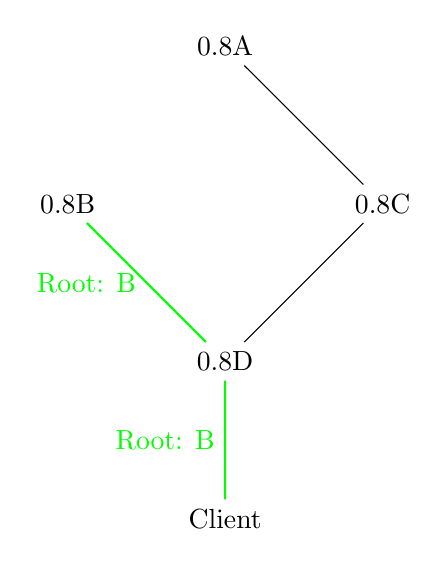
\begin{tikzpicture}
            \node (A) at (4,8) {\switch{0.8}{A}};
            \node (B) at (2,6) {\switch{0.8}{B}};
            \node (C) at (6,6) {\switch{0.8}{C}};
            \node (D) at (4,4) {\switch{0.8}{D}};
            \node (client) at (4,2) {Client};

            \draw
            (A) -- (C)
            (C) -- (D);

            \draw[green, thick]
            (B) -- node [left] {Root: B} ++ (D)
            (D) -- node [left] {Root: B} ++ (client);
        \end{tikzpicture}
        \caption{Correct information}
    \end{subfigure}
    \hspace{1cm}
    \begin{subfigure}[b]{0.4\textwidth}
        \begin{tikzpicture}
            \node (A) at (4,8) {\switch{0.8}{A}};
            \node (B) at (2,6) {\switch{0.8}{B}};
            \node (C) at (6,6) {\switch{0.8}{C}};
            \node (D) at (4,4) {\switch{0.8}{D}};
            \node (client) at (4,2) {Client};

            \draw
            (A) -- (C)
            (C) -- (D);

            \draw[red, thick]
            (B) -- node [left] {Root: A} ++ (D)
            (D) -- node [left] {Root: A} ++ (client);

            \draw[red, thick, dashed]
            (A) -- node [left] {Root: A} ++ (B);

            \begin{customlegend}[legend cell align=left, legend entries={Connection, Assumptions:, Correct, Incorrect, Non Existing}, legend style={at={(8.2,8.7)},font=\footnotesize}]
                \addlegendimage{}
                \addlegendimage{white}
                \addlegendimage{green}
                \addlegendimage{red}
                \addlegendimage{red, dashed}
            \end{customlegend}
        \end{tikzpicture}
        \caption{False assumption}
    \end{subfigure}

    \caption{An example case of false assumptions about network structure}
    \label{fig:false_example}
\end{figure}
We did not find an alternate way to gather information about connections in the network, so we tried to reduce errors created by our method.
To this end we combine information gathered by multiple clients to identify and remove false information.
If a client makes a false assumption about a bridge, the message age for that bridge will be lower than its actual messge age.
An example can be seen in Figure~\ref{fig:message_ages}.
\begin{figure}[h]
    \begin{subfigure}[b]{0.4\textwidth}
        \begin{tikzpicture}
            \node (A) at (4,8) {\switch{0.8}{A:0}};
            \node (B) at (2,6) {\switch{0.8}{B:1}};
            \node (C) at (6,6) {\switch{0.8}{C:1}};
            \node (D) at (4,4) {\switch{0.8}{D:2}};
            \node (client) at (4,2) {Client};

            \draw
            (A) -- (C)
            (C) -- (D)
            (B) -- (D)
            (D) -- (client);

            \draw [red, thick, dashed]
            (A) -- (B);

        \end{tikzpicture}
        \caption{Assumed message ages}
    \end{subfigure}
    \hspace{1cm}
    \begin{subfigure}[b]{0.4\textwidth}
        \begin{tikzpicture}
            \node (A) at (4,8) {\switch{0.8}{A: 0}};
            \node (B) at (2,6) {\switch{0.8}{B: 3}};
            \node (C) at (6,6) {\switch{0.8}{C: 1}};
            \node (D) at (4,4) {\switch{0.8}{D: 2}};
            \node (client) at (4,2) {Client};

            \draw
            (A) -- (C)
            (C) -- (D)
            (B) -- (D)
            (D) -- (client);

        \end{tikzpicture}
        \caption{Actual message ages}
    \end{subfigure}

    \caption{Assumed and actual message ages}
    \label{fig:message_ages}
\end{figure}
By comparing bridge data from multiple clients we can find and remove bridges whose message age is lower than it should be.
The code for doing this is shown in Listing~\ref{lst:remove}.
\lstinputlisting[caption=Removing Incorrect Bridge Data, label=lst:remove]{../listings/stp/remove.c} %TODO: maybe do better formatting
The bridges are removed from the vector they each are in.
This way any connection information that is not proven wrong is retained.
\section{Combining the data}
\label{combining_data}
After false information is removed, the bridge data is combined into one SpanningTree object.
Creating large SpanningTree objects is done in multiple steps.
First, we combine the bridge vectors to individual trees.
These trees each represent a path from a client to the root.
After the individual trees are obtained, we combine the ones with the same root.
The code for this can be seen in Listing~\ref{lst:combine}.
\lstinputlisting[caption=Combining the Bridge Data, label=lst:combine]{../listings/stp/combination.c}
Combining the individual trees into one is done using the operator we overloaded.
This operator executes a recursive tree combine, which is shown in Figure~\ref{lst:treeCombine}.
\lstinputlisting[caption=Recursive Tree Combination Algorithm, label=lst:treeCombine]{../listings/stp/treeAdd.cpp}

\section{Visualization}
\tool\ generates \textit{.tex} files containing \textit{TikZ} graphs.
Nodes in these graphs contain the bridge data.
Edges show the (assumed) connections in the topology.
Node information is displayed in the format \textit{priority, system id extension - MAC address, message age}.
For cases where \tool\ has no knowledge of the path to the root, empty nodes are used.
These can be seen as gaps in the final output.
Figure~\ref{fig:viz_example} shows an example.
\begin{figure}[h]
    %TODO: change to new output format
    \centering
    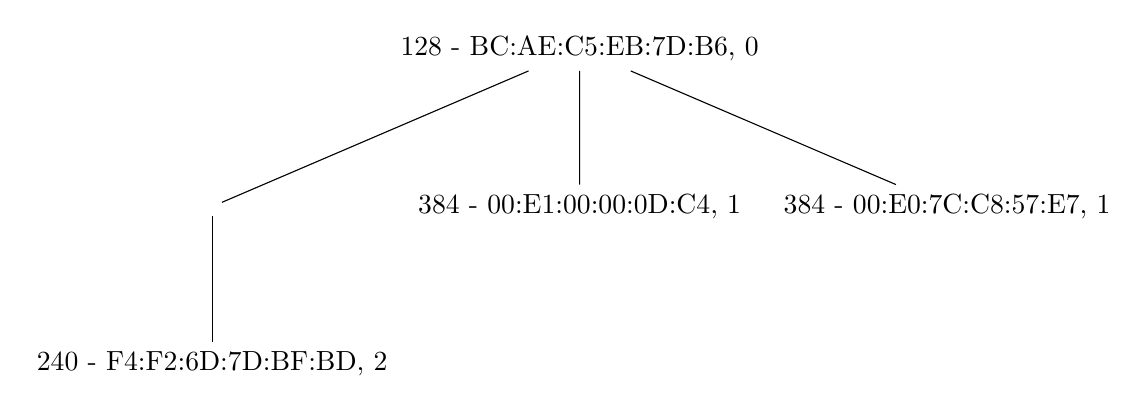
\begin{tikzpicture}
        \node (0) at (7.000000,20) {128 - BC:AE:C5:EB:7D:B6, 0};
        \node (1) at (2.333333,18) {};
        \node (2) at (2.333333,16) {240 - F4:F2:6D:7D:BF:BD, 2};
        \draw (1) -- (2);
        \node (3) at (7.000000,18) {384 - 00:E1:00:00:0D:C4, 1};
        \node (4) at (11.666667,18) {384 - 00:E0:7C:C8:57:E7, 1};
        \draw 
        (0) -- (1)
        (0) -- (3)
        (0) -- (4);
    \end{tikzpicture}
    \caption{An example for \tool\ output}
    \label{fig:viz_example}
\end{figure}

The output is generated using a recursive function in the \textbf{SpanningTree} class.
Our code for this is rather confusing when first read, so we decided to split it into multiple listings, allowing for clearer explanations.
No code is skipped between the listings, so combining Listings~\ref{lst:output1}-\ref{lst:output4} would yield the original function.
To make it easier to follow we also did not modify any indentations.
Viewing the code together with the raw \LaTeX\ output makes it much clearer, so Listing~\ref{lst:raw} shows the output for Figure~\ref{fig:viz_example}
\lstinputlisting[caption=\textit{.tex} code for Figure~\ref{fig:viz_example}, label=lst:raw]{../listings/output.tex}
For an explanation on TikZ keywords please refer to the section on TikZ (Section~\ref{tikz}).

\lstinputlisting[caption={TikZ conversion function, part 1}, label=lst:output1]{../listings/stp/output1.cpp}
The \textit{lowerX}, \textit{upperX}, \textit{y} and \textit{yStep} parameters are used to calculate the position for the current root, as well as the subtrees.
\textit{OldMessageAge} is used to discern whether or not \tool\ needs to draw empty nodes.
As we use incrementing IDs to draw connections between the nodes (see Listing~\ref{lst:raw}), we need to \textit{index} to pass the current index.
This function is executed recursively until the current \textbf{SpanningTree} has no children, so the first step is always to calculate the position of the current root (see Listing~\ref{lst:spanningTree}).
The previous child index calculation will be discussed in the explanation for Listing~\ref{lst:output4}.

\lstinputlisting[caption={TikZ conversion function, part 2}, label=lst:output2]{../listings/stp/output2.cpp}
If there is an unknown bridge between the current root and the previous one, we draw an empty node to visualize this.
After the empty node is drawn, the same function will be called with increased \textit{y} coordinate, because the current root has not been handled yet.
We also know that the ID will be the current index plus 1.
With these informations we can write the command for drawing the edge beforehand.
Note that we include newlines to keep the output readable.
As the returned string is a C++ \textbf{std::string} we use the \textbf{\textbackslash n} escape sequence.

\lstinputlisting[caption={Tikz conversion function, part 3}, label=lst:output3]{../listings/stp/output3.cpp}
Here we draw the node for the current root.
To calculate the amounts of horizontal space the subtrees can use, we use their respective maximum width.
This width is calculated using the functions shown in Listing~\ref{lst:maxWidth}.
For subtree spacing we simply use the relation between the width of the full tree and the width of all children.
In Listing~\ref{lst:output3} we see the reason why we have to return a pair of \textbf{string} and \textbf{int}.
As it would be rather expensive to check for the number of empty nodes that need to be drawn beforehand (this would double the required computational effort), we return the last used index as well.
This eliminates ID conflicts.
To keep drawing the nodes and edges in blocks, we use multiple loops for drawing them.
This leads to edges being drawn in "layers", as edges from a node to all its children are drawn at once.
Only "deep" topologies (with a spanning tree of depth > 3) are affected.%TODO: include deep example

\lstinputlisting[caption={Tikz conversion function, part 4}, label=lst:output4]{../listings/stp/output4.cpp}
Listing~\ref{lst:output4} shows how we draw edges between nodes and their children.
We use the same method of accessing the indices as in Listing~\ref{lst:output3}.
Before returning we set the the returned \textit{int} half of the pair to the largest index used by a recursive call.

\lstinputlisting[caption=Calculating the maximum width of a tree, label=lst:maxWidth]{../listings/stp/maxWidth.cpp}

\section{Installation \& Usage}
\tool\ was written in C++ and requires a compiler capable of C++11.
Usage of the included Makefile is strongly advised.
We included the version of \textit{jsoncpp} we used, so it does not need to be downloaded.
The client requires an installation of the \textit{pcap} development library to compile, and the regular library to run.
Available build targets are \textbf{client}, \textbf{server}, \textbf{parser} for single components and \textbf{all} for all components.
An \textbf{install} target for global installation is not provided.
\subsection*{Client Launch Parameters}
\paragraph{-if \textit{inputFile}} is  used to specify the name of an input file which is written in \textit{.pcapng} format.
If specified packets will not be captured live, but instead taken from the input file.
For easier usage with this parameter, launching the server with a higher timeout duration is recommended.
The server will remove data from this client, as it is not programmed to resend data taken from input files.
%TODO: change client to send file data only once?

\paragraph{-of \textit{outputFile}} is used to specify a different output file.
Output files are used for logging data.
Logging directly to \textbf{STDOUT} is currently not possible.

\paragraph{--no-connect / -nc} will stop the client from connecting to a server.
This was used for debugging the client, but remains in the current version.

\paragraph{-h \textit{hostname}} will tell the client which hostname to connect to.
IPv4 addresses in dot notation, as well as hostnames (including URLs) are accepted.
For more information on accepted formats please refer to the manual page for \textbf{gethostbyname}.

\paragraph{-p \textit{port}} specifies the port on which to connect.

\paragraph{-dn \textit{deviceName}} tells the client the device name of the interface to use.
The names can be obtained using commands such as \textbf{ifconfig} or \textbf{ip addr show}.

\subsection*{Server Launch Parameters}
\paragraph{-p \textit{port}} specifies the port to listen on.

\paragraph{-of \textit{outputFile}} specifies the filename for the output file, which is used for logging incoming data, as well as the current state.

\paragraph{-np} disables the creation of a \textit{.pid} file containing the process id.
In cases the server is meant to be launched automatically in the background this file provides an easy means of accessing the process id.

\paragraph{-t \textit{timeout}} tells the server how large the timeout time should be before removing a client's data.

\subsection*{Parser Launch Parameters}
\paragraph{-p \textit{port}} specifies the port to connect on.

\paragraph{-h \textit{hostname}} specifies the hostname to connect to.

\paragraph{-pw \textit{pictureWidth}} specifies the width of the resulting TikZ picture.
Note that if a width of 20cm is specified but only 10 are used, the picture will be snipped automatically

\paragraph{-ph \textit{pictureHeigth}} specifies the height of the resulting TikZ picture.
The same snipping occurs as for the width.

\paragraph{-s \textit{yStep}} defines the vertical distance between layers.

\subsection*{Default Parameters}
\paragraph{Client} parameters default to the following values:
\begin{itemize}
    \item \textbf{-if}: defaults to nothing, live capture is used
    \item \textbf{-of}: client.log in the current working directory
    \item \textbf{-nc}: not set
    \item \textbf{-h}: \textit{localhost}
    \item \textbf{-p}: 80
    \item \textbf{-dn}: first named device
\end{itemize}

\paragraph{Server} parameters default as follows:
\begin{itemize}
    \item \textbf{-p}: 80
    \item \textbf{-of}: server.log in the current working directory
    \item \textbf{-np}: not set
    \item \textbf{-t}: 10
\end{itemize}

\paragraph{Parser} parameters default to the following values:
\begin{itemize}
    \item \textbf{-p}: 80
    \item \textbf{-h}: \textit{localhost}
    \item \textbf{-s}: 2
    \item \textbf{-ph}: 20
    \item \textbf{-pw}: 14
\end{itemize}

\subsection*{Configuration Files}
The binaries all create configuration files with their current configuration if none exist.
On subsequent launches they will take their configuration from these files.
Command line parameters take precedence over configuration files, which in turn take precedence over default parameters.
